\documentclass[sigconf,nonacm,prologue,table]{acmart}
\usepackage{listings}

%% labels
%% sections:    "sec"
%% definitions: "def"
%% equations:   "eq"
%% figures:     "fig"
%% tables:      "tab"

%% packages
\usepackage{amsmath}
% \usepackage{pgfplots}
\usepackage{subcaption}
\usepackage{commath}
\usepackage[utf8]{inputenc}
% \usetikzlibrary{positioning, arrows.meta, shapes, calc}
%% \usepackage{tikz}
\usepackage{graphicx}
\usepackage{afterpage}

\pagenumbering{arabic}

%% hide ACM reference
\settopmatter{printacmref=false}

%% hide copyright
\renewcommand\footnotetextcopyrightpermission[1]{}

%% \pagestyle{plain}
\settopmatter{printfolios=true}

% \numberwithin{equation}{section}

% \theoremstyle{definition}
% \newtheorem{definition}{Definition}

% \theoremstyle{remark}
% \newtheorem*{remark}{Remark}

\begin{document}
\title{USD+ Whitepaper}
\subtitle{Aug 2024}
\date{Aug 2024}

\author{Jake Timothy}
\affiliation{}
\email{jake@dinari.com}

\begin{teaserfigure}
\caption*{
    \hspace{\textwidth}
    }
\end{teaserfigure}

\renewcommand{\shortauthors}{Timothy}

\begin{abstract}

    The USD+ protocol provides a convenient USD denominated way for people to earn low risk yield on chain. The primary protocol token (USD+) provides a clear unit of value and accumulates generated yield.

\end{abstract}

\maketitle

\section{Introduction}
\label{sec:introduction}

The USD+ token is a dollar denominated digital token. The protocol mints and redeems 1 USD+ token for \$ 1 USD value. USD+ tokens earn yield generated by the protocol.

The protocol earns yield by investing the funds and tokens used to mint USD+ tokens into fixed income assets, initially short duration US Treasury bills. 

\section{System Architecture} 
\label{sec:system}

\subsection{USD+ Token}

The USD+ Token is an ERC20 compliant fungible token. It implements administrative minting, burning, and rebasing functions to manage the supply of the token.

\subsection{Wrapped USD+ Token}

The Wrapped USD+ Token is an ERC4626 compliant fungible token vault. USD+ is deposited into the Wrapped USD+ smart contract in order to facilitate interoperability and composability with common blockchain applications and accounting systems. Users can withdraw USD+ from the Wrapped USD+ contract at any time.

\subsection{Reserves Vault}

The Reserves Vault is an onchain account holding the onchain portion of the assets backing the value of USD+ including yield generating tokenized assets. The Reserves Vault will primary invest in short duration US Treasury bills directly or indirectly.

\subsection{Minter}

The Minter handles USD+ minting. It maintains list of approved payment tokens and their price oracles. USD+ is always minted at 1 USD+ = 1 USD. When a user calls `deposit` on the Minter smart contract, the deposit is processed immediately, sending payment token to the Reserves Vault and minting USD+ at the current oracle price for that payment token.

\subsection{Redeemer}

The Redeemer handles USD+ burning. It also maintains a list of approved payment tokens and their price oracles. USD+ is always burned at 1 USD+ = 1 USD. Burning USD+ and sending payment token to the user is a two step process. There may be delays that take up to 2 days to process when liquidating the underlying investments and converting to the requested payment token for distribution. When a user calls `requestRedeem` on the Redeemer smart contract, the USD+ is escrowed on the Redeemer contract and the payment token price is taken at that time and the payment token amount is fixed for that request. The protocol will then fulfill the request if payment token is available in the Reserves Vault, or rebalance assets and tokens to make payment token available before fulfilling the redemption request.

% \begin{figure}
%     \centering
%     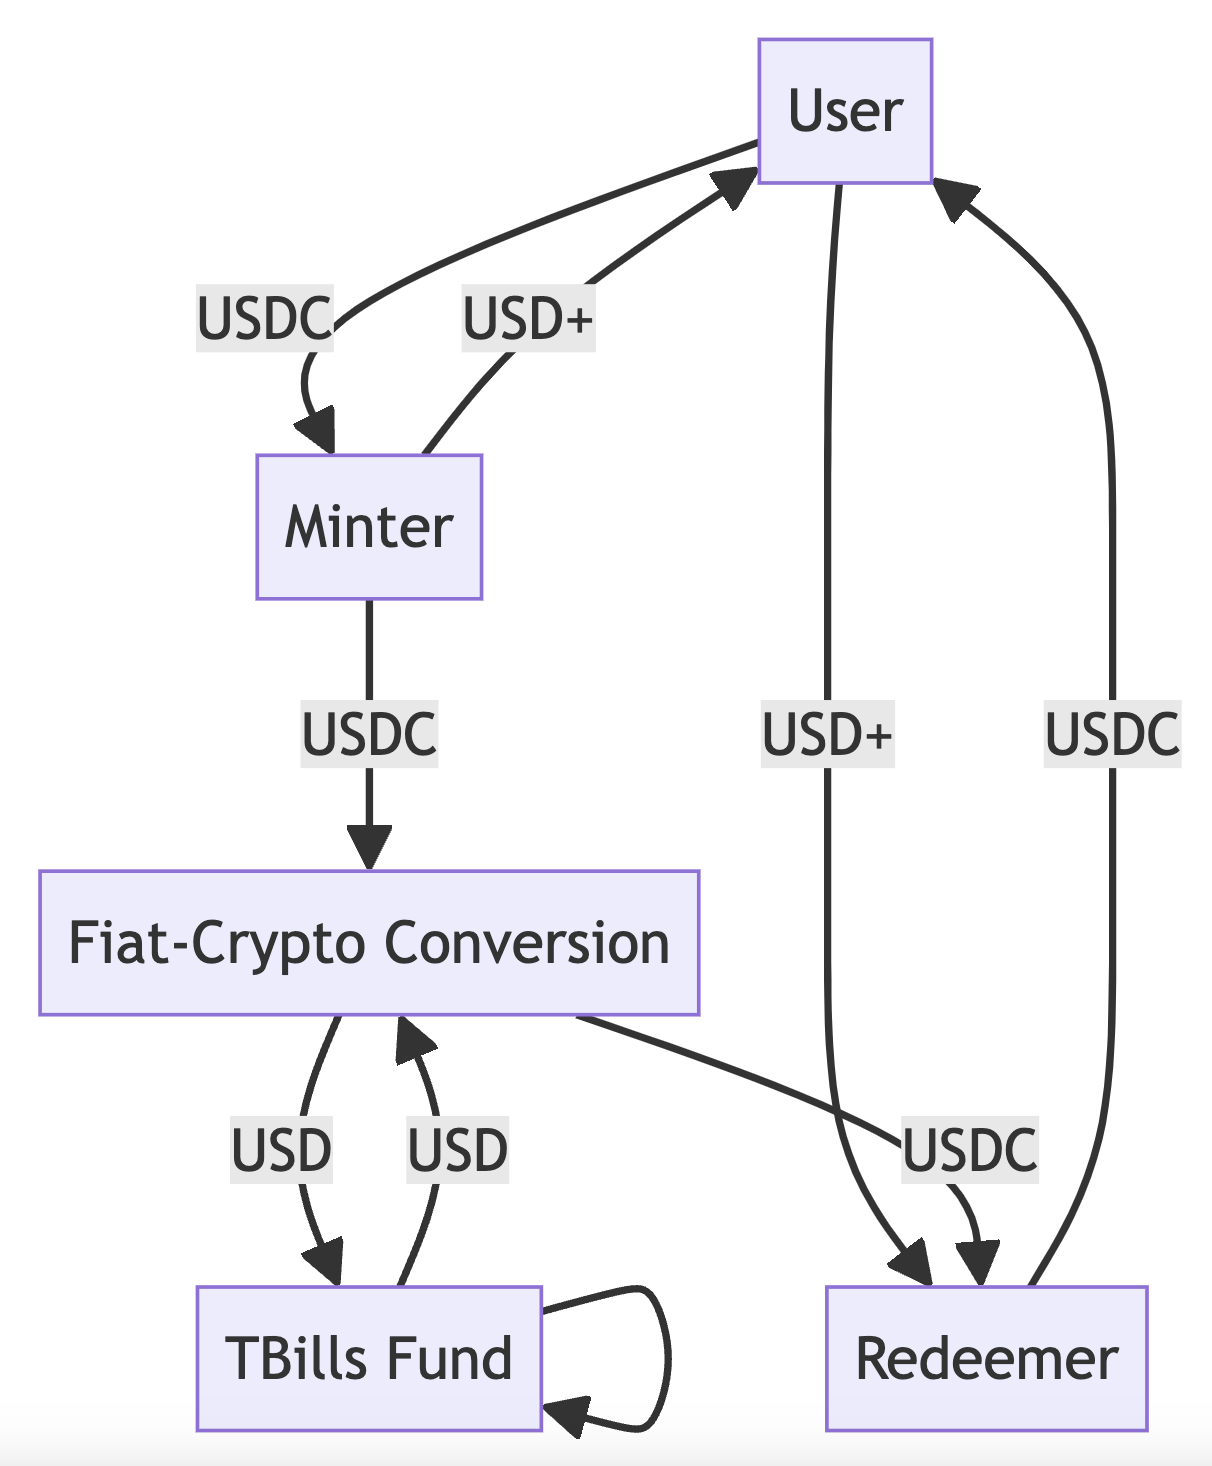
\includegraphics[width = \textwidth]{flowchart}
%     \caption{System Overview}
%     \label{fig:system}
% \end{figure}


\section{Earning Yield}
\label{sec:lockups}

USD+ earns yield from the performance of the underlying fixed income assets. When the investments generate yield, the distribution is automatically reinvested increasing the total value of the assets backing USD+. That increase in value is shared with USD+ holders by "rebasing" or updating the amount of USD+ held in each account. This rebase is performed as a single action on the blockchain.

\section{Summary}

The USD+ protocol provides a convenient and effective access point to low risk yield on chain. The protocol is designed to be simple and transparent, and to provide a clear and stable value for users. It is also designed to be flexible and to be able to adapt to changing market conditions and user needs.

% \bibliographystyle{ACM-Reference-Format}
% \bibliography{whitepaper}

\section*{Disclaimer}

This paper is for general information purposes only. It does not constitute investment advice or a recommendation or solicitation to buy or sell any investment and should not be used in the evaluation of the merits of making any investment decision. It should not be relied upon for accounting, legal or tax advice or investment recommendations.  This paper reflects current opinions of the authors. The opinions reflected herein are subject to change without being updated. 

\end{document}
